\section{Site pressure and boundary gluing}
\label{sec:pressure}

Throughout this section, $0<q<1$ is fixed, and we put
\[
 u=1-q,\qquad t=q^{-1}.
\]
The graphs are finite and their edge odds are nonnegative and finite,
unless a limiting identification is specified. The basic pressure and
rooted-connection arguments do not require planarity; the cofacial
comparisons additionally use a fixed plane embedding. Together they
provide the restricted connection comparisons used in the geometric
arguments. The proof has three stages. We first obtain nonnegative
coefficients for a site-pressure expansion. Those coefficients give a
rooted multiset representation of connections to an added wire. Finally,
we combine the resulting comparisons with an extremal planar search to
glue connections between interlacing boundary electrodes.
Every result in this section follows from these finite hypotheses.

For a graph $H=(V,E)$, write
\begin{equation}
 Z_H=\sum_{A\subset E}q^{k(V,A)}v_A,
 \qquad v_A=\prod_{e\in A}v_e,
 \label{pressure:partition}
\end{equation}
and let $\PP_H$ be the corresponding FK law. Components include isolated
vertices. A preexisting wire is treated as a vertex identification before
this notation is applied. Thus a vertex of $H$ may represent several
vertices of an earlier physical graph; a path in $H$ need not lift to a
physical path in that earlier graph. We write $\EE_0$ for independent bond
percolation with opening probabilities $v_e/(1+v_e)$ on the same graph.
Loops factor independently out of \eqref{pressure:partition}. Parallel
edges can be replaced by a single edge of odds
$\prod_e(1+v_e)-1$ whenever only connectivity is at issue.

\subsection{A positive expansion of the site pressure}

For a vertex set $C$, put $x_C=\prod_{a\in C}x_a$ and define
\begin{equation}
 F_H(x)=\EE_0\prod_{C\text{ component of }(V,A)}(1-u x_C).
 \label{pressure:polynomial}
\end{equation}
This is a polynomial, affine in each site variable, with $F_H(0)=1$.
The component product is a site-variable form of the external-field
FK expansion in \cite[Section~6]{Sokal2001ComplexZeros}; the hub
calculation below identifies these variables.
At $x=\one_V$, every component contributes $q$, so
\[
 F_H(\one_V)=\frac{Z_H}{\prod_{e\in E(H)}(1+v_e)}.
\]
Site values in $(0,1]^V$ also have a partition-function interpretation.
Adjoin a new vertex $o$ to $H$ and finitely many links from vertices of
$H$ to $o$, allowing several links at a site. For this specialization put
\[
 s_i=\prod_{h:\,i-o}(1+v_h),\qquad x_i=s_i^{-1},
 \qquad s_C=\prod_{i\in C}s_i,
\]
where an empty product is one. For a fixed original open graph, summing
the hub links at a component $C$ gives weight $q$ if none is open and
weight $s_C-1$ otherwise, with one further global factor $q$ for the
hub component. Consequently
\begin{equation}
 Z_{H+o}=q\left(\prod_{e\in E(H)}(1+v_e)\right)
              \left(\prod_{i\in V}s_i\right)F_H(1/s).
 \label{pressure:hub-partition}
\end{equation}
We will use the next theorem to control how this partition function
changes with the hub links. Its coefficient signs will also turn a
derivative at a vertex into a probability law.

\begin{theorem}[Positive site pressure]
\label{thm:pressure}
There are coefficients $c_m\ge0$, indexed by the nonzero multiindices
$m\in\Z_{\ge0}^{V}$, such that
\begin{equation}
 -\log F_H(x)=\sum_{m\ne0}c_m x^m,
 \qquad x^m=\prod_{i\in V}x_i^{m_i}.
 \label{pressure:series}
\end{equation}
The series converges absolutely on a polydisk containing the closed
unit polydisk in its interior. If $c_m>0$, the support
$\{i:m_i>0\}$ is connected in $H$.
\end{theorem}

\begin{proof}
We first identify the squarefree coefficients of $F_H$, then the signs
of its logarithmic coefficients, and finally the convergence domain.
The sign argument uses labeled copies of vertices: an auxiliary
cancellation removes repeated types before the logarithm is taken.

\paragraph{The coefficients of the site polynomial.}
Discard loops and combine parallel edges, so that $H$ is simple. Set
\[
 \gamma_i=\prod_{e\ni i}(1+v_e)^{-1},\qquad y_i=\gamma_i x_i.
\]
Selecting a collection of components in
\eqref{pressure:polynomial} with union $T$ forces every edge between $T$
and its complement to be closed. Summing all edges in the complement
therefore shows that the coefficient of $y_T$ is
\begin{equation}
 W(T)=\prod_{e\in E(H[T])}(1+v_e)
       \sum_{A\subset E(H[T])}v_A(-u)^{k(T,A)}.
 \label{pressure:squarefree}
\end{equation}
Indeed, the factors $\gamma_i$ count each internal edge twice, whereas
the percolation normalization counts it once. This accounts for the
first product in \eqref{pressure:squarefree}. Coefficients with a
repeated variable vanish.

\paragraph{Connected structures and logarithmic signs.}
To take the logarithm, use a finite set $U$ of labeled elements, each
carrying a type in $V$; there are $m_i$ elements of type $i$. Repeated
types are needed because a logarithm need not be squarefree, even when
$F_H$ is. The two ordinary edge sets below represent, respectively,
the partition sum and the extra product in
\eqref{pressure:squarefree}; hard edges cancel repeated types before
the connected-structure restriction is imposed. Between
elements of distinct adjacent types allow an ordinary edge with the
corresponding odds $v_e$. Between elements of the same type allow a
hard edge. For a subset $J\subset U$, independently choose two sets
$A,B$ of ordinary edges and a set $L$ of hard edges, and give the
resulting structure weight
\begin{equation}
 v_Av_B(-u)^{k(J,A)}(-1)^{|L|}.
 \label{pressure:structure-weight}
\end{equation}
If a type repeats in $J$, summation over a possible hard edge cancels
the full sum. If no type repeats, summation over $B$ gives the first
product in \eqref{pressure:squarefree}, and the full sum is $W(T)$.
Consequently the sum of \eqref{pressure:structure-weight} is the mixed
derivative of $F_H$ at zero in the labeled $y$-slots $J$.

The weight factors over the connected components of $A\cup B\cup L$.
In particular the number of $A$-components is additive over those
components. Decomposing every structure according to its partition
into connected components proves the labeled exponential formula in
this setting: the mixed derivative of $\log F_H$ in the slots $U$ is
the same sum restricted to structures with $A\cup B\cup L$ connected.
This is an identity of formal series; no convergence assertion is
being used yet.
For the corresponding connected-graph logarithm in the hard-core gas,
see \cite[Proposition~2.1]{ScottSokal2005RepulsiveGas}.

We group this connected sum by the ordinary-edge union $D=A\cup B$.
If $(U,D)$ has $b$ components, the ordinary-edge sum has sign
$(-1)^b$ or vanishes, while the connected hard-edge sum has sign
$(-1)^{b-1}$ or vanishes. Their product gives the required nonpositive
sign for the logarithmic derivative.

For fixed $D$, an edge of $D\setminus A$ must
belong to $B$ and contributes $v_e$. An edge of $A$ may or may not
belong to $B$, and contributes $v_e(1+v_e)$. Thus summing over $A,B$
with union $D$ gives
\begin{equation}
 v_D\prod_{D_0}Z(D_0;-u,1+v),
 \qquad
 Z(G;s,w)=\sum_{R\subset E(G)}s^{k(V(G),R)}w_R,
 \label{pressure:fixed-union}
\end{equation}
where $D_0$ ranges over the connected components of $(U,D)$.

For every connected graph $G$ and weights $w_e\ge1$, one has
\begin{equation}
 Z(G;-u,w)<0.
 \label{pressure:negative-partition}
\end{equation}
This is a special case of \cite[Theorem~4.4]{JacksonSokal2009TutteZeros},
where the result is attributed to Dong. Here is a direct induction
for the present weights, including multigraphs. A loop contributes a
positive factor $1+w_e$. A bridge can be contracted at the positive
factor $w_e-u$. For an edge that is neither a loop nor a bridge,
deletion and contraction both leave connected graphs, and
\[
 Z(G;-u,w)=Z(G\setminus e;-u,w)+w_e Z(G/e;-u,w)
\]
is the sum of two negative terms. The initial graph with one vertex
and no edges has partition function $-u$. This proves
\eqref{pressure:negative-partition}.

It remains to sum the hard edges, subject to $D\cup L$ being connected.
If a possible hard edge lies within a $D$-component, its two choices
cancel because it has no effect on this connectivity requirement.
Otherwise contract all $D$-components. The hard-edge sum becomes
\[
 \sum_{L:\,([b],L)\text{ connected}}(-1)^{|L|},
 \qquad b=k(U,D),
\]
on a hard multigraph with $b$ vertices. This sum is either zero or has
sign $(-1)^{b-1}$. To see this directly, loops cancel, disconnected
graphs have sum zero, and the deletion-minus-contraction recursion
preserves the asserted sign; the one-vertex graph has value one.
The $b$ factors in \eqref{pressure:fixed-union} have sign $(-1)^b$.
Their product with the hard-edge sum is therefore nonpositive.
Each contribution grouped by the ordinary union $D$, after summing
the hard edges, is therefore nonpositive. Dividing by the positive
factorials of the multiplicities
and rescaling from $y$ to $x$ proves $c_m\ge0$.

A connected structure on the labeled elements projects to a connected
set of vertex types: hard edges only join equal types and ordinary
edges project to edges of $H$. This proves the assertion about support.
The hard-edge sign and connected-support conclusions are the
repulsive-gas principles of
\cite[Propositions~2.8--2.9]{ScottSokal2005RepulsiveGas} after the
ordinary-union regrouping above; the argument here proves them directly
for this site polynomial.

\paragraph{Convergence beyond the unit polydisk.}
The preceding arguments are formal coefficient identities. To use their
derivatives as probabilities, we must also justify convergence at
$x_i=1$. The following direct nonnegative-series argument is the finite form of
the convergence principle in \cite[Theorem~2.10]{ScottSokal2005RepulsiveGas}.
For $x\in[0,1]^V$, every factor in
\eqref{pressure:polynomial} is at least $q$, so $F_H(x)>0$.
The diagonal series
\[
 G(z)=\sum_{m\ne0}c_m z^{|m|}
\]
has nonnegative coefficients and a positive radius of convergence,
because it initially equals $-\log F_H(z,\ldots,z)$ near zero.
Suppose its radius $R$ were finite and at most one. Positivity of
$F_H$ on the real interval gives an analytic continuation of this
germ through a neighborhood of $R$. For each derivative order,
monotone convergence as $z\uparrow R$ identifies the nonnegative
coefficient sum at $R$ with the corresponding finite derivative
$G^{(j)}(R)$. For small $h>0$, Taylor expansion at $R$ and summation
of nonnegative terms would then give
\[
 \sum_{m\ne0}c_m(R+h)^{|m|}
   =\sum_{j\ge0}\frac{G^{(j)}(R)}{j!}h^j<\infty,
\]
contrary to the definition of $R$. Thus $R>1$ (or $R=\infty$).
For any $1<r<R$, the diagonal sum bounds the absolute sum on
$|x_i|\le r$. The negative of the series exponentiates to $F_H$, since this
identity holds near zero and hence throughout the polydisk.
The series agrees with the real negative logarithm on the unit cube.
\end{proof}

We record two consequences of the proof that will be useful when
comparing pressure coefficients in different local graphs.

\begin{lemma}[Locality and identification of zero sites]
\label{pressure:coefficient-locality}
For a simple graph and a fixed multiindex $m$, write
\begin{equation}
 c_m=\left(\prod_i\gamma_i^{m_i}\right)b_m.
 \label{pressure:incident-factors}
\end{equation}
Then $b_m\ge0$ depends only on the induced graph on $\supp(m)$ and
its odds, and is nondecreasing in each of these odds. Thus decreasing
the incident products $\prod_{e\ni i}(1+v_e)$ at support vertices,
with the induced graph unchanged, cannot decrease $c_m$.

If variables on a set $S$ are fixed to zero, identifying any groups
of vertices within $S$ does not change $F_H$ as a polynomial in the
remaining variables, provided the new identified vertices also have
site variable zero. In particular all pressure coefficients whose
support avoids $S$ remain unchanged under these identifications.
\end{lemma}

\begin{proof}
The labeled construction above involves only types in $\supp(m)$.
After the factors in \eqref{pressure:incident-factors} are extracted,
$b_m$ is a finite sum of nonnegative contributions, one for each
ordinary union $D$. Apart from a nonnegative integer from the
hard-edge sum and a positive factorial denominator, each contribution
is
\[
 v_D\prod_{D_0}\bigl[-Z(D_0;-u,1+v)\bigr].
\]
For a connected graph, differentiating $Z$ with respect to a nonloop
weight gives the partition function of its contraction, which is
negative by \eqref{pressure:negative-partition}; differentiating in
a loop weight gives the partition function with that loop removed,
also negative. Hence every factor $-Z$ is nondecreasing in the edge
weights. Adding an allowed induced edge merely adds nonnegative
terms as well. This proves the first assertion, with parallel edges
combined before applying it.

For the second assertion, fix the states of the original edges.
Every component meeting $S$ has factor one in
\eqref{pressure:polynomial}. Identifying vertices in $S$ only merges
some of these components and leaves all other components unchanged.
The product of factors is therefore unchanged for every edge state.
The independent edge law is unchanged as well; edges that become
loops can be retained. Taking expectations proves the polynomial
identity, and taking its logarithm at zero proves the coefficient
identity.
\end{proof}

\subsection{Hub links and restricted correlation inequalities}

Return to the augmented graph and the products $s_i$ in
\eqref{pressure:hub-partition}. The pressure expansion now gives
comparison inequalities for its incident links.

\begin{lemma}[Adjacent and cofacial Rayleigh inequalities]
\label{lem:adjacent-rayleigh}
In every finite FK graph with $0<q<1$, two distinct edges incident to
a common vertex have nonpositive covariance of their opening
indicators. In a plane graph the same conclusion holds for two
distinct edges incident to a common face. Both statements remain
valid after deleting or contracting any other edges.
\end{lemma}

\begin{proof}
Regard the common vertex as $o$, remove it to obtain $H$, and regard
its incident nonloop edges as hub links. By
\eqref{pressure:hub-partition} and Theorem~\ref{thm:pressure}, the part
of $\log Z_{H+o}$ depending on those links is
\begin{equation}
 \sum_h\log(1+v_h)
 -\sum_{m\ne0}c_m\prod_h(1+v_h)^{-m_{i(h)}}.
 \label{pressure:hub-log}
\end{equation}
Every monomial in the second sum has nonnegative mixed derivative
in the odds of two distinct links, including links at the same site.
The first sum has mixed derivative zero. Absolute convergence on a
larger polydisk justifies termwise differentiation, including at
zero link odds by continuity. Thus
$\partial_{v_e}\partial_{v_f}\log Z\le0$ for distinct incident edges.
For positive odds,
\begin{equation}
 \partial_{v_e}\partial_{v_f}\log Z
  =\frac{\Cov(\one_{\{e\text{ open}\}},
                     \one_{\{f\text{ open}\}})}{v_ev_f}.
 \label{pressure:rayleigh-derivative}
\end{equation}
Loops are independent of all other edge states and cause no exception.

For the plane statement, complementary dual edges have odds $q/v_e$.
Two primal edges on a common face become two dual edges at a common
vertex. Complementing both opening indicators preserves their
covariance, so the adjacent inequality in the dual gives the claimed
cofacial inequality. Zero odds and contraction limits follow by
continuity of finite partition functions after removal of their
common leading factors.
\end{proof}

\begin{lemma}[Monotonicity of tested network connections]
\label{pressure:network-monotonicity}
Let $a,o$ be vertices in a finite graph. Adding or strengthening an
edge incident to $o$ does not decrease $\PP(a\leftrightarrow o)$. The same
holds in a plane graph if the added edge and an auxiliary connection
test edge from $a$ to $o$ can be drawn cofacially in the graph
containing both edges. In particular, adding vertices to a terminal
by identification does not decrease its connection probability to another
fixed terminal.

For any three vertices $a,b,o$,
\begin{equation}
 \PP(a\leftrightarrow o,\ b\leftrightarrow o)
 \ge \PP(a\leftrightarrow o)\PP(b\leftrightarrow o).
 \label{pressure:root-correlation}
\end{equation}
\end{lemma}

\begin{proof}
Add a distinct auxiliary edge $f$ between $a$ and $o$, initially of
odds zero. Its logarithmic partition derivative is
\begin{equation}
 \left.\partial_{v_f}\log Z\right|_{v_f=0}
 =\PP(a\leftrightarrow o)+q^{-1}\PP(a\not\leftrightarrow o)
 =q^{-1}-(q^{-1}-1)\PP(a\leftrightarrow o).
 \label{pressure:test-edge}
\end{equation}
The mixed derivative with respect to the strengthened edge is
nonpositive by Lemma~\ref{lem:adjacent-rayleigh}. Because
$q^{-1}-1>0$, the tested connection probability is nondecreasing.
The cofacial argument is identical. Sending incident auxiliary odds
to infinity proves the terminal-identification assertion.

For \eqref{pressure:root-correlation}, induct on the number of edges,
discarding loops. If no nonloop edge touches $o$, both tested events
are constant. Otherwise condition on an edge $e$ incident to $o$.
The conditional laws are FK on the deletion and contraction minors,
and their conditional covariance is nonnegative by induction.
Moreover, each of the two conditional means is at least as large
when $e$ is open as when it is closed: vary its odds from zero to
infinity in the connection monotonicity just proved. The covariance
of these two conditional means is consequently nonnegative. The
conditional covariance identity proves the induction step. Cases
in which a tested vertex is contracted to $o$ simply make its event
constant one.
\end{proof}

The pressure coefficients encode more than derivative signs. After
weighting by the multiplicity at a root, they form a probability law
on connected vertex multisets. Wiring a set then becomes the event
that the multiset meets it. In particular, unions of target sets can
be compared in one fixed probability space, even though their FK laws
have different wires. The unrooted coefficients $c_m$ have a second
role: their mass over multisets meeting a set gives its full-wiring
log gain, up to the single constant for the surviving wired component.
The lemma records both forms.

\begin{lemma}[Rooted coverage representation]
\label{lem:rooted}
For $a\in V$, the numbers
\begin{equation}
 \mu_H^a(m)=\frac q u m_a c_m
 \label{pressure:rooted-law}
\end{equation}
define a probability law on finite nonempty vertex multisets with
connected support containing $a$. In the graph with hub links above,
\begin{equation}
 \PP_{H+o}(a\not\leftrightarrow o)
   =\sum_m\mu_H^a(m)x^m.
 \label{pressure:rooted-nonconnection}
\end{equation}
If $S\subseteq V$ is nonempty, let $H/S$ identify precisely the
vertices of $S$, with no other new identifications. Then
\begin{equation}
 \PP_{H/S}(a\leftrightarrow S)
  =\mu_H^a\{m:\supp(m)\cap S\ne\varnothing\}.
 \label{pressure:rooted-hit}
\end{equation}
Here $S$ on the left denotes the collapsed vertex. Equivalently,
adjoin a fresh hub with exactly one infinite-odds link from each site
of $S$ and no other incident links.
Any identifications already represented in $H$ are retained.
Writing $k_S(A)$ for the number of open components meeting $S$,
\begin{equation}
 K_H(S):=\log\EE_H t^{k_S}
  =\sum_{\supp(m)\cap S\ne\varnothing}c_m.
 \label{pressure:coverage}
\end{equation}
In particular $K_H$ is a nonnegative coverage function,
$K_H(\{a\})=\log t$, and
\begin{equation}
 K_H(S)+K_H(T)-K_H(S\cup T)
 =\sum_{\substack{\supp(m)\cap S\ne\varnothing\\
                   \supp(m)\cap T\ne\varnothing}}c_m\ge0.
 \label{pressure:double-coverage}
\end{equation}
\end{lemma}

\begin{proof}
Differentiate \eqref{pressure:hub-partition} with respect to $s_a$:
\begin{equation}
 s_a\partial_{s_a}\log Z_{H+o}
       =1+\sum_m m_a c_m x^m.
 \label{pressure:hub-derivative}
\end{equation}
This derivative has a second interpretation. Conditional on the
original open graph, the component $C_a$ has hub-link factor
$s_{C_a}-u$. Its contribution to the derivative is
\[
 \frac{s_{C_a}}{s_{C_a}-u}
   =1+\frac{u}{s_{C_a}-u},
\]
while its conditional probability of having no hub link is
$q/(s_{C_a}-u)$. Averaging under the marginal original-edge law of
the augmented graph and comparing with
\eqref{pressure:hub-derivative} proves
\eqref{pressure:rooted-nonconnection}. At $s_i=1$ for every $i$, the
hub is isolated, so the right side equals one. Nonnegativity and the
support assertion now follow from Theorem~\ref{thm:pressure}.
For the $H/S$ specialization, adjoin a fresh hub with links only at
$S$ and send their odds to infinity. Then $x_i=0$ on $S$ and $x_i=1$
elsewhere, giving \eqref{pressure:rooted-hit}, including when $a\in S$.

For \eqref{pressure:coverage}, put $x_i=\one_{\{i\notin S\}}$ in
\eqref{pressure:polynomial}. A component meeting $S$ then contributes
one instead of q. Hence
\[
 \frac{F_H(\one_{V\setminus S})}{F_H(\one_V)}
       =\EE_H q^{-k_S}.
\]
Take logarithms and use \eqref{pressure:series}. For a singleton,
$k_{\{a\}}=1$ in every configuration, so $K_H(\{a\})=\log t$.
The final identity is the inclusion-exclusion identity for the two
support-hitting events in the nonnegative sum.
\end{proof}

The rooted law controls connection probabilities, while
\eqref{pressure:coverage} measures the gain from full boundary wiring.
We first record two quantitative forms of the connection statement.
Adjoin a fresh vertex $o$ with exactly one odds-$v$ link to each site
of $I\subseteq V$ and no other incident links. Then
\begin{equation}
 \PP(a\leftrightarrow o)
 =\EE_{\mu_H^a}\bigl[1-(1+v)^{-N_I}\bigr],
 \qquad N_I=\sum_{i\in I}m_i.
 \label{pressure:finite-spokes}
\end{equation}
In particular this probability is between
$\frac{v}{1+v}\mu_H^a(N_I>0)$ and $\mu_H^a(N_I>0)$, uniformly in
the number of links. Second, if $A$ and $T$ are nonempty disjoint
vertex sets, define
\begin{equation}
 g_H(A,T)=\PP_{H/(A,T)}(A\leftrightarrow T),
 \label{pressure:network-g}
\end{equation}
where each of the two sets is separately identified. In this law,
connection is equivalent to an open path in the represented base
graph $H$ from a vertex of $A$ to a vertex of $T$, using no hop from
either of these two new wires. Indeed a shortest quotient connection has
a segment from its last departure from the first wire to its first
arrival at the second wire with no wire hop in between.
If the edges of $H$ are physical edges and each vertex is a single
physical vertex, this is an actual physical path. If $H$ arose from
an earlier physical graph by other identifications, the path may pass
through one of those quotient vertices. Recovering a path in the earlier
physical graph then requires an explicitly available open connection
between the incidences used at each such class.
Apply \eqref{pressure:rooted-hit} on the fixed graph $H/A$ with root
the collapsed $A$. The union bound under this single multiset law
gives
\begin{equation}
 g_H(A,T_1\cup T_2)\le g_H(A,T_1)+g_H(A,T_2),
 \label{pressure:subadditivity}
\end{equation}
whenever both target sets are disjoint from $A$. They need not be
disjoint from each other. Symmetry gives the corresponding assertion
for the first terminal.

\subsection{A no-hit comparison without planarity}

It is important not to confuse the preceding network monotonicity
with the effect of wiring the target of an as-yet unwired hit event.
For that operation the comparison has the opposite direction.

\begin{lemma}[Wiring an unwired target]
\label{pressure:general-no-hit}
Let $a$ be a vertex and $S$ a nonempty vertex set in any finite graph
$H$. The probability that the open component of $a$ meets $S$ is at
least its probability after all vertices of $S$ have been identified:
\begin{equation}
 \PP_H(a\leftrightarrow S)
   \ge \PP_{H/S}(a\leftrightarrow S).
 \label{pressure:general-hit-comparison}
\end{equation}
The original graph may already contain identifications, including a
wire represented by the root $a$.
\end{lemma}

\begin{proof}
If $a\in S$, both probabilities are one. Otherwise induct on the
number of edges, ignoring independent loops. If no nonloop edge is
incident to $S$, both probabilities are zero. Choose a nonloop edge
$e$ with endpoint $s\in S$. Write $\mu=\PP_H$, $\nu=\PP_{H/S}$, and
let $\alpha,\beta$ be their respective probabilities that $e$ is open.
To form $H/S$, add auxiliary links from $s$ to all other vertices of
$S$ and send their odds to infinity. Every such link is incident to
$e$. Lemma~\ref{lem:adjacent-rayleigh} therefore gives
\begin{equation}
 \alpha\ge\beta.
 \label{pressure:target-edge-marginal}
\end{equation}

For $j=0,1$, let $h_j$ and $\widetilde h_j$ be the conditional hit
probabilities under $\mu$ and $\nu$, respectively, given the state
$j$ of $e$. Conditional FK laws are deletion and contraction minors.
Identification of $S$ commutes with both operations, with its image
used after contraction. The induction hypothesis therefore gives
$h_j\ge\widetilde h_j$. If $e$ becomes a loop in $H/S$, its state is
independent of the hit event and $\widetilde h_1=\widetilde h_0$.
Otherwise it is incident to the collapsed target terminal, and
Lemma~\ref{pressure:network-monotonicity} gives
$\widetilde h_1\ge\widetilde h_0$. Thus
\begin{align*}
 \PP_H(a\leftrightarrow S)
 &=\alpha h_1+(1-\alpha)h_0\\
 &\ge\alpha\widetilde h_1+(1-\alpha)\widetilde h_0\\
 &\ge\beta\widetilde h_1+(1-\beta)\widetilde h_0
  =\PP_{H/S}(a\leftrightarrow S).
\end{align*}
If contraction brings $a$ into the image of $S$, the corresponding
conditional probabilities are both one. Zero odds are obtained by
continuity, or by deleting those edges at the start.
\end{proof}

\subsection{Cofacial partition gains}

We next isolate the partition-function form of cofacial comparison.
It will also justify erasing an exposed component in later cap
arguments. A plane graph here has a fixed tame embedding; incidences
on different banks of a cut are distinct incidences.

\begin{lemma}[Cofacial gain and exposed erasure]
\label{pressure:cofacial-gain}
Let $X$ be a finite collection of auxiliary edges between vertices
of a plane graph $K$, and let $h$ be an original edge. Suppose that, in the
drawing containing all these edges, $h$ and each edge of $X$ are
cofacial. For fixed nonnegative auxiliary odds, the gain
\begin{equation}
 \frac{Z_{K+X}}{Z_K}
 \label{pressure:gain}
\end{equation}
is nonincreasing in the odds of $h$.

In particular, suppose $B\ne\varnothing$, $X$ is an auxiliary tree
with vertex set exactly $B$, and the drawing of $K+X$ has a face incident to a
vertex $a$ and to every edge of $X$. Let $U$ be a connected vertex
set in $K$ containing $a$ and disjoint from $B$. Then
\begin{equation}
 \EE_{K-U}t^{k_B-1}\ge\EE_K t^{k_B-1}.
 \label{pressure:erasure-gain}
\end{equation}
The same conclusion holds if $U$ is the vertex set of an open
component containing $a$.
\end{lemma}

\begin{proof}
Raise the auxiliary odds successively from zero to their prescribed
values. The logarithm of \eqref{pressure:gain} is the sum of the
integrals of $\partial_{v_f}\log Z$ for $f\in X$ during these changes.
Its derivative with respect to the odds of $h$ is nonpositive by the
cofacial assertion of Lemma~\ref{lem:adjacent-rayleigh}. This proves
the first statement; all embeddings are kept fixed, even when an
edge has odds zero.

For the second, delete the edges of $K$ incident to $U$ in an exposed
order. Start at the face sector incident to $a$. Once one sector at
a vertex of $U$ is exposed, delete its incident edges successively
around its cyclic fan, thereby enlarging the same face. An edge
leading to another vertex of $U$ exposes a sector there. A spanning
tree of the connected set $U$ ensures that this procedure reaches
every vertex of $U$. All original edges incident to $U$ can therefore
be deleted, and every edge at its deletion borders the expanding
face. The edges of $X$ remain on its boundary, because none touches
$U$ and deleting an edge never splits a face. If the deleted edge
has the same face on both sides, that face remains available along
both banks; otherwise its two incident faces merge. A loop can be removed
without affecting any gain. At each step the first part of the
lemma shows that the auxiliary-edge gain cannot decrease. Isolated
vertices left in $U$ contribute the same factors to numerator and
denominator and can be discarded.

Finally send every auxiliary odds to infinity and divide the gain
by their product. For a fixed original edge state, the tree $X$
identifies all $k_B$ components meeting $B$, changing the cluster
count by $-(k_B-1)$. The limiting gain is consequently
$\EE_K q^{1-k_B}$, and after erasure it is
$\EE_{K-U}q^{1-k_B}$. This proves
\eqref{pressure:erasure-gain}. An open component is connected in the
underlying graph, so it satisfies the same geometric hypothesis.
\end{proof}

For example, if $a$ does not hit $B$ and one conditions on its
component vertex set $U$, the unremoved graph has FK law on $K-U$.
The weight for additionally wiring $B$ is $t^{k_B-1}$.
Equation~\eqref{pressure:erasure-gain} says that its conditional mean
on this no-hit event is at least its unconditional mean. Weighting
by it therefore does not decrease the no-hit probability. This gives a
planar partition-gain proof of the special case of
Lemma~\ref{pressure:general-no-hit} used below, as well as the more
explicit erasure comparison needed for boundary partitions.

\subsection{Interlacing boundary connections}

Let $H$ be embedded in a topological closed disk. An electrode is a
nonempty set of boundary vertices contained in a specified closed
boundary arc. We require that its vertices are accessible from the
exterior on that arc: an arbitrarily small outward extension can
reach them without crossing the graph. Separate electrodes below
lie on disjoint such arcs; unmarked vertices may occupy the gaps.
This convention includes ordinary lattice polygons and their cut
surfaces.

Figure~\ref{fig:interlacing} shows the separation geometry in an
ordinary physical graph. The probability inequality requires the conditional argument below,
since its two input probabilities have different boundary wires.
\begin{figure}[tbp]
\centering
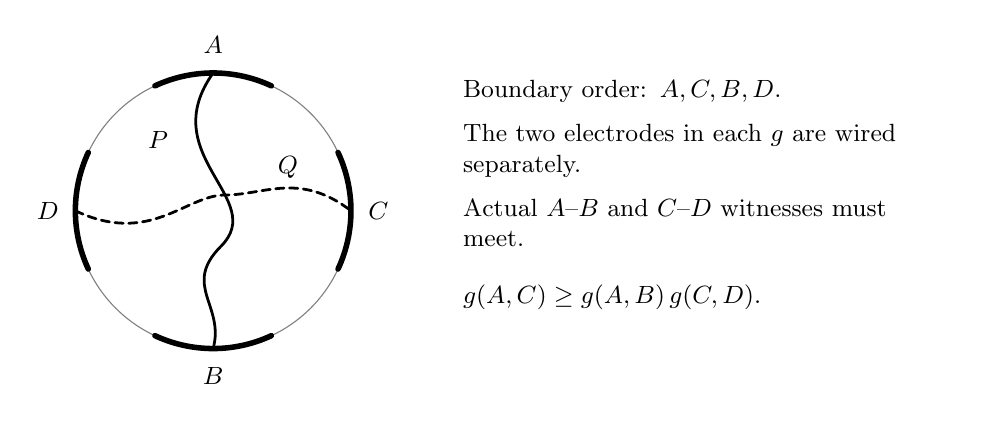
\begin{tikzpicture}[x=1cm,y=1cm,font=\small,line cap=round,line join=round]
  \draw[gray] (0,0) circle (1.75);
  \foreach \start/\finish/\name/\angle in {65/115/A/90,-25/25/C/0,-115/-65/B/-90,155/205/D/180} {
    \draw[line width=2pt] (\start:1.75) arc (\start:\finish:1.75);
    \node at (\angle:2.1) {$\name$};
  }
  \draw[line width=1pt] (0,1.75) .. controls (-.75,.7) and (.7,.15) .. (.1,-.45)
    .. controls (-.4,-.95) and (.15,-1.2) .. (0,-1.75);
  \draw[densely dashed,line width=1pt] (-1.75,0) .. controls (-.8,-.45) and (-.35,.2) .. (.15,.2)
    .. controls (.65,.2) and (1.1,.5) .. (1.75,0);
  \node[fill=white,inner sep=1.5pt] at (-.7,.9) {$P$};
  \node[fill=white,inner sep=1.5pt] at (.95,.55) {$Q$};
  \node[align=left,anchor=west,text width=6.1cm] at (3.05,.6)
    {Boundary order: $A,C,B,D$.\\[5pt]
     The two electrodes in each $g$ are wired separately.\\[5pt]
     Actual $A$--$B$ and $C$--$D$ witnesses must meet.};
  \node[anchor=west] at (3.05,-1.1)
    {$g(A,C)\geq g(A,B)\,g(C,D)$.};
\end{tikzpicture}
\caption{The topology behind interlacing gluing. Thick boundary arcs mark the four electrode sets, not a common four-wire law: each probability $g$ wires only its own two electrodes. The curves $P,Q$ illustrate actual witnesses and their forced meeting, not simultaneous events under one boundary condition. The probability inequality uses the restricted comparison and the extremal exploration in Lemma~\ref{lem:interlacing}, not positive association or independence.}
\label{fig:interlacing}
\end{figure}


\begin{lemma}[Interlacing gluing]
\label{lem:interlacing}
Suppose four electrodes occur in cyclic order $A,C,B,D$ on the
boundary of one disk. With $g_H$ defined by
\eqref{pressure:network-g},
\begin{equation}
 g_H(A,C)\ge g_H(A,B)\,g_H(C,D).
 \label{pressure:interlacing}
\end{equation}
The edge odds may be arbitrary nonnegative finite numbers. The disk
embedding and electrode-access assumptions are imposed after any
preexisting identifications. Apart from the two wires specified in
each $g_H$, there are no further abstract ties between distinct
vertices of this embedded graph.
All path witnesses in the proof use edges of this represented graph
$H$ before the electrode wires are added. If $H$ is a quotient of an
earlier physical graph, the statement alone does not assert that those
paths lift to physical paths in the earlier graph.
\end{lemma}

\begin{proof}
Our base law has $A,C$ separately wired. First we compare an
$A$--$B$ path in $H$ with a network hit. We then expose
an extremal such witness and compare the uninspected $C$ side with
the separate $C,D$ network. The two comparisons will give the two
factors on the right of \eqref{pressure:interlacing}.

\paragraph{From a network hit to a path in $H$.}
Denote the collapsed $A$ by $a$. Lemma~\ref{pressure:general-no-hit} says that the
probability that the component of $a$ hits the as-yet unwired set
$B$ is at least the corresponding probability when $B$ is also
wired. In the latter law, its $A$-to-$B$ connection probability is
at least $g_H(A,B)$. Indeed, realize the additional $C$ wire by a
chain of exterior links along its arc. This chain and a test edge
joining exposed representatives of $A$ and $B$, drawn farther
outside, are cofacial. Apply
Lemma~\ref{pressure:network-monotonicity} and then take the wire
limits.

Let $S$ be the event that there is an open path in $H$ from
$A$ to $B$, using no electrode identification as a hop. If $a$ hits $B$
in the $A,C$ quotient but $S$ fails, a shortcut through $C$ must have
been used. The initial part of such a quotient path, through its
first visit to $C$ and after its last departure from $A$, is an
open $A$-to-$C$ path in $H$. Jumps within $A$ alone cannot produce
a hit of $B$ without an open $A$-to-$B$ path in $H$. Consequently, writing
$T=\{A\leftrightarrow C\}$ in the current law,
\begin{equation}
 \PP(S)+\PP(T\cap S^c)\ge g_H(A,B).
 \label{pressure:physical-hit}
\end{equation}

\paragraph{A measured separator with an uninspected side.}
We now expose such an $A$-to-$B$ path from the $D$ side, leaving
its $C$ side uninspected. Here are explicit details, including
boundary contacts. Only for the search, add disjoint exterior spokes
from $A$ to a terminal $s$ and from $B$ to a terminal $s'$. The
spokes are declared traversable by the search; they are not sampled
edges and do not add any FK identifications. Choose a slightly
enlarged disk with $s,s'$ on its boundary so that the spoke interiors
are inside it. The electrode accessibility assumption lets each
$C$ vertex retain access to the boundary arc on one side of $s,s'$
and each $D$ vertex retain access to the other, without crossing a
spoke or a graph edge. Call these the $C$ and $D$ sides.

Split the exterior face at $s,s'$ and seed the search only at its
$D$-side face. Query an edge from a reached face and enter its opposite
face only when that primal edge is closed. Process the edges incident
to reached faces until the $C$ side is reached or no such unqueried
edge remains. Empty regions of the drawing can be subdivided by dummy
closed edges, whose dual crossings are free; this merely formalizes
the face search. The finite planar path/cut alternative
says that it reaches the other side exactly when there is no open
$s$-to-$s'$ path. One proof is to trace the boundary of the primal
vertices reachable from $s$: in the absence of the connection,
this boundary contains a separating closed-primal dual crosscut.
Conversely, such a crosscut intersects every primal connection.
An open $s$-to-$s'$ path is equivalent to $S$.

On $S$, the explored dual component is exhausted on the $D$ side.
Every edge on its frontier was queried and is open if it prevents
further dual exploration. Setting every unqueried edge of $H$
closed cannot enlarge the explored dual component, since all
edges incident to it have already been queried. The path/cut
alternative therefore still supplies an open $s$-to-$s'$ path in
this modified configuration. Choose a simple such path by a fixed
deterministic rule. It consists of queried open edges and exactly
one initial and one final spoke, so its portion $\gamma$ in $H$
is an open $A$-to-$B$ path determined by the exploration
record.

No reached face is strictly on the $C$ side of this simple path:
the explored dual component starts on the other side and cannot
cross an open primal path or an exterior spoke. Hence no edge of $H$
whose interior is strictly on the $C$ side was queried. If
$\gamma$ meets $C$, event $T$ already holds. Otherwise all $C$
vertices lie on its $C$ side, while all $D$ vertices lie on its
$D$ side or on the path. These assertions follow also for original
boundary contacts by using the retained exterior access curves in
the enlarged disk.

\paragraph{The conditional connection comparison.}
Condition on a successful search record for which $\gamma$ does
not meet $C$. Finite FK domain Markov gives the ordinary FK law on
the unqueried graph with identifications induced by the queried
open connections and the original $A,C$ wires. Restricting to the
right, or $C$-side, subgraph, this means that $\gamma$ is wired,
any $A$ vertices on that side are tied to it, and $C$ is wired
separately. The rest attaches only through the path or that same
$A$ wire. There are no additional ties from the fictitious $B$
spokes: they were only a device for defining the search. Integrating
the other side therefore introduces no further boundary condition.

Dropping the extra $A$ vertices from the first terminal cannot increase
its tested connection probability by
Lemma~\ref{pressure:network-monotonicity}. The conditional chance
of $T$ is consequently at least the pure $\gamma$-to-$C$ network
probability in this right subgraph. To compare that probability
with $g_H(C,D)$, start instead in the full $C,D$-wired graph and add
all vertices of $\gamma$ to the $D$ terminal. This cannot decrease its
connection probability to $C$. After this identification, the
entire left subgraph, including $D$, attaches to the right subgraph
through one wired vertex. FK partition functions factor across a
one-vertex attachment: if $H_1,H_2$ meet at just a wired vertex,
then $k(A_1\cup A_2)=k(A_1)+k(A_2)-1$, so the extra partition
factor cancels from all probabilities determined on $H_1$.
Thus the enlarged-terminal probability in the full graph is exactly
the pure $\gamma$-to-$C$ probability on the right. It follows that
\begin{equation}
 \PP(T\mid\text{successful search record})\ge g_H(C,D).
 \label{pressure:conditional-interlacing}
\end{equation}
The same inequality is automatic if $\gamma$ already meets $C$.

This decomposition remains valid if the simple path touches the
original boundary several times: work in the enlarged disk,
assign off-path edge interiors to their respective sides, and
observe that the only shared graph vertices are path vertices.
Any loops created at the wire are independent and cancel.
The search is adaptive but queries only determined edge states;
conditioning on a record is exactly a finite domain Markov
conditioning and imposes no event on the unqueried right edges.

Average \eqref{pressure:conditional-interlacing} over the successful
records. Since $g_H(C,D)\le1$, \eqref{pressure:physical-hit} yields
\begin{align*}
 g_H(A,C)=\PP(T)
 &\ge g_H(C,D)\PP(S)+\PP(T\cap S^c)\\
 &\ge g_H(C,D)\bigl[\PP(S)+\PP(T\cap S^c)\bigr]\\
 &\ge g_H(C,D)g_H(A,B),
\end{align*}
as required.
\end{proof}

\begin{remark}[Scope of the comparisons]
\label{pressure:scope}
The inequalities above concern tested network connections, rooted
connection events, or specified cofacial changes. They assert
neither positive association for arbitrary increasing events nor
stochastic monotonicity under arbitrary boundary wiring.
Lemma~\ref{lem:interlacing} is a statement about four interlacing
electrodes in a single disk, not an overlapping-rectangle gluing
principle or an arbitrary-boundary-condition crossing estimate.
\end{remark}
